\section{Flow Plots}



 First, we examine the `Pre-Fish Negative controls'. We plot the Sample.replicate number on the x-axis, and the transformed CT (TCT) of the associated eight technical replicates on the y-axis. These plots correspond to tanks which had just been filled by the infill pipe, and no additional water had been allowed to flow through the tank.


\begin{figure}[H]
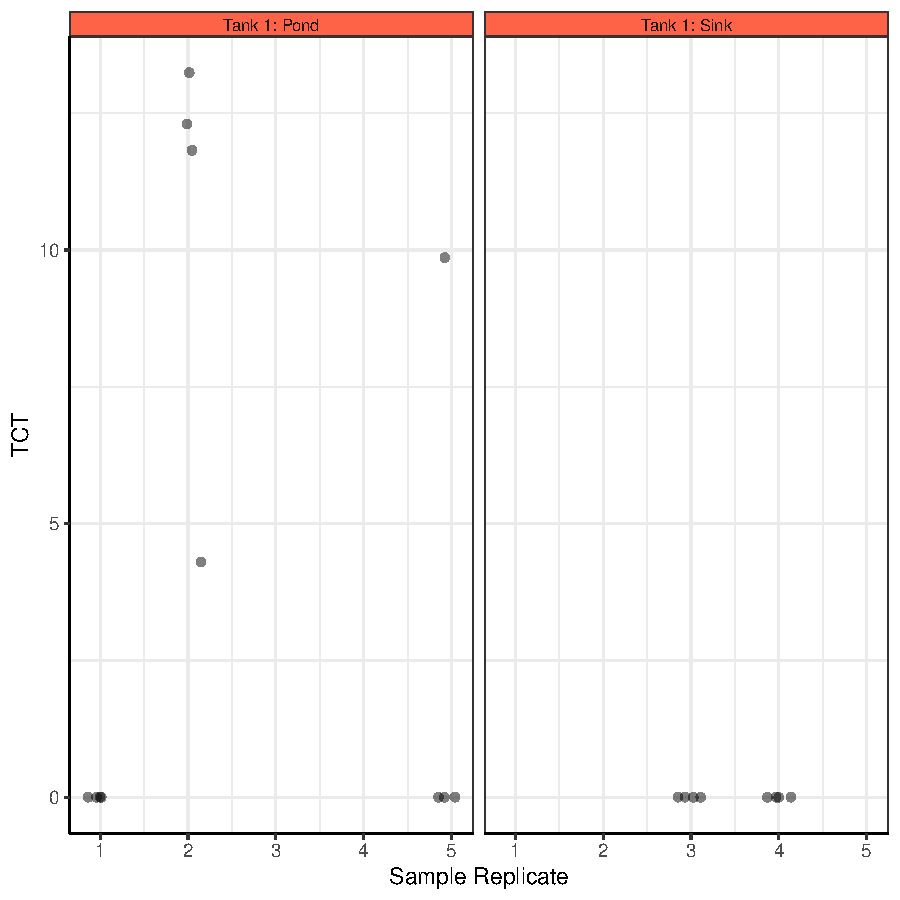
\includegraphics[scale=0.8]{Chapter4Images/pondandsink.pdf}
\caption{Transformed CT values obtained from samples taken from pond and sink water. Samples were taken from a small tank, tank 1.}
\label{fig:sinkandpond}
\end{figure}

Figure~\ref{fig:sinkandpond} are the plots of TCT values obtained from the hatchery sink and the hatchery pond. The water was transferred to tank 1 where sample replicates were then obtained. The goal of these measurements was to observe possible background hatchery signal of Coho eDNA. While the sink water showed no sign of Coho eDNA, the samples from the pond did indicate presence of Coho.




\begin{table}[H]
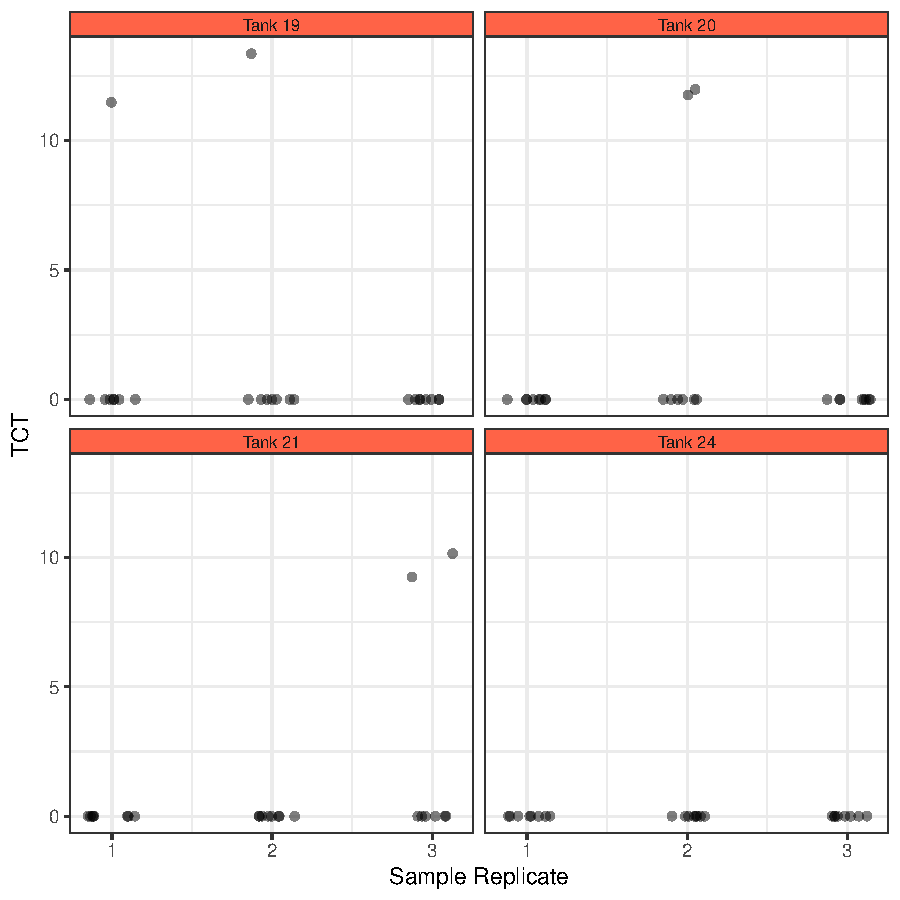
\includegraphics[scale=0.8]{Chapter4Images/zerofishtct.pdf}
\caption{Transformed CT values obtained from pre-fish negative controls. }
\label{lab:flowzerofish}
\end{table}

Table~\ref{lab:flowzerofish} are the TCT plots obtained from the tanks before the fish were added. The samples help to measure a hatchery background signal of Coho eDNA. Most samples indicate no presence of Coho eDNA, although there exist several outliers. This may indicate that the hatchery water itself contains trace amounts of Coho eDNA.




\begin{figure}[H]
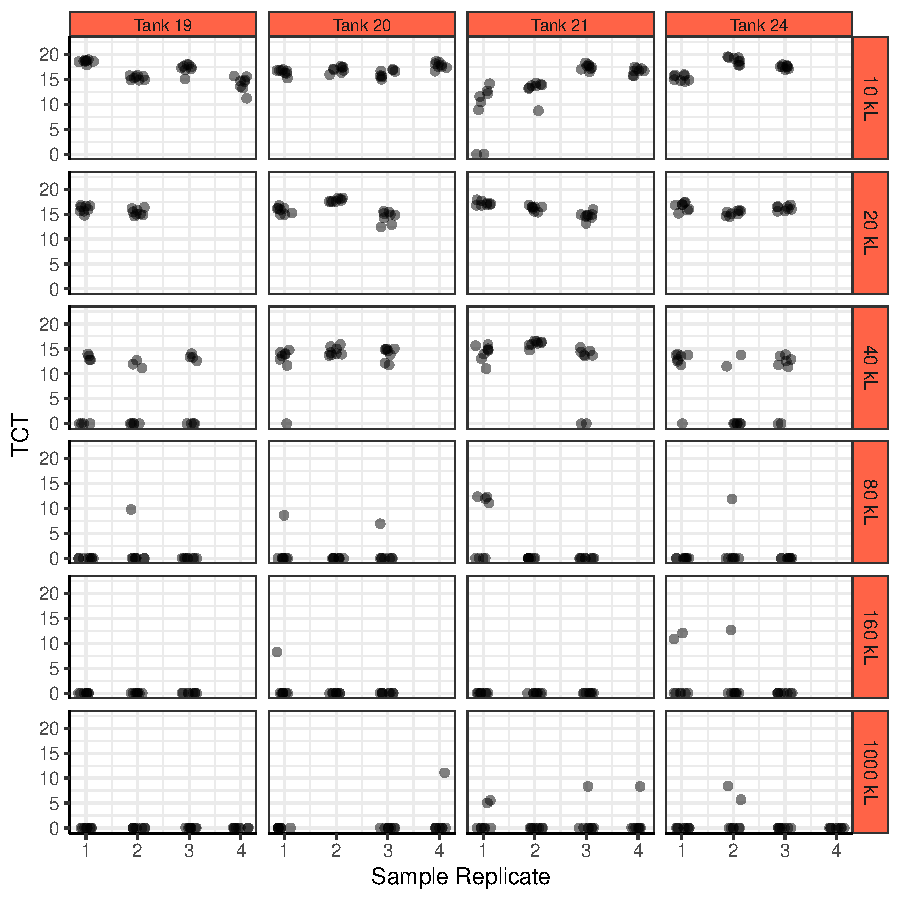
\includegraphics{Chapter4Images/finalflowplots.pdf}
\caption{Transformed CT values obtained from samples taken from each tank at differing levels of dilution.}
\label{fig:finalflowplot}
\end{figure}





Table~\ref{fig:finalflowplot} are the TCT plots obtained from the tanks after the indicated levels of dilution. Note that the 10kL corresponds to samples that were taken right after the fish were removed (prior to dilution). When only 20kL of water had been allowed to flow through the tank, we consistently detected eDNA. At 40kL of flow, we still had consistent detection, but the number of non-detects began to increase more significantly. By the time we reach 80kL, detection of Coho eDNA was no longer consistent. Presence of Coho eDNA was not being picked up, except in a small number of cases. For flows greater than 80kL, we are no longer consistently detecting Coho eDNA. However, there does exist the rare detection of Coho eDNA at even the higher levels of flow. This may be due to the background noise in the hatchery water that we previously discussed.

